Below are the results of the band-pass filter. The measured frequencies and amplitudes are then plotted on a bode plot.
\vspace{1cm}
\begin{adjustwidth}{-2.5 cm}{-2.5 cm}\centering\begin{threeparttable}[!htb]
        \scriptsize
        \begin{tabular}{lrrrrr}\toprule
            \textbf{Input Voltage(in V)} & \textbf{Output Voltage(in V)} & \textbf{Phase(in deg)} & \textbf{Frequency(in Hz)} & \textbf{Amplitude(in dB)} \\\midrule
            10.4                         & 2.92                          & 73.4                   & 50                        & -11.03                    \\
            10.4                         & 5.2                           & 53                     & 100                       & -6.02                     \\
            10                           & 7.68                          & 38.8                   & 200                       & -2.29                     \\
            10                           & 9.44                          & 16.5                   & 500                       & -0.50                     \\
            10.4                         & 10                            & 4.32                   & 1000                      & -0.34                     \\
            10.9                         & 10.5                          & -4.04                  & 2000                      & -0.32                     \\
            11.6                         & 10.5                          & -19.4                  & 5000                      & -0.87                     \\
            11.6                         & 9.12                          & -37.7                  & 10000                     & -2.09                     \\
            11.6                         & 6.4                           & -55                    & 20000                     & -5.17                     \\
            11.6                         & 2.92                          & -73.4                  & 50000                     & -11.98                    \\
            12.4                         & 1.54                          & -80.5                  & 100000                    & -18.12                    \\
            \bottomrule
        \end{tabular}
        \caption{The measured input voltage, output voltage, phase, and amplitude ratio in dB}
    \end{threeparttable}\end{adjustwidth}

\pagebreak
We then plot the frequency response on the bode plot as shown below:

\begin{figure}[H]
    \centering
    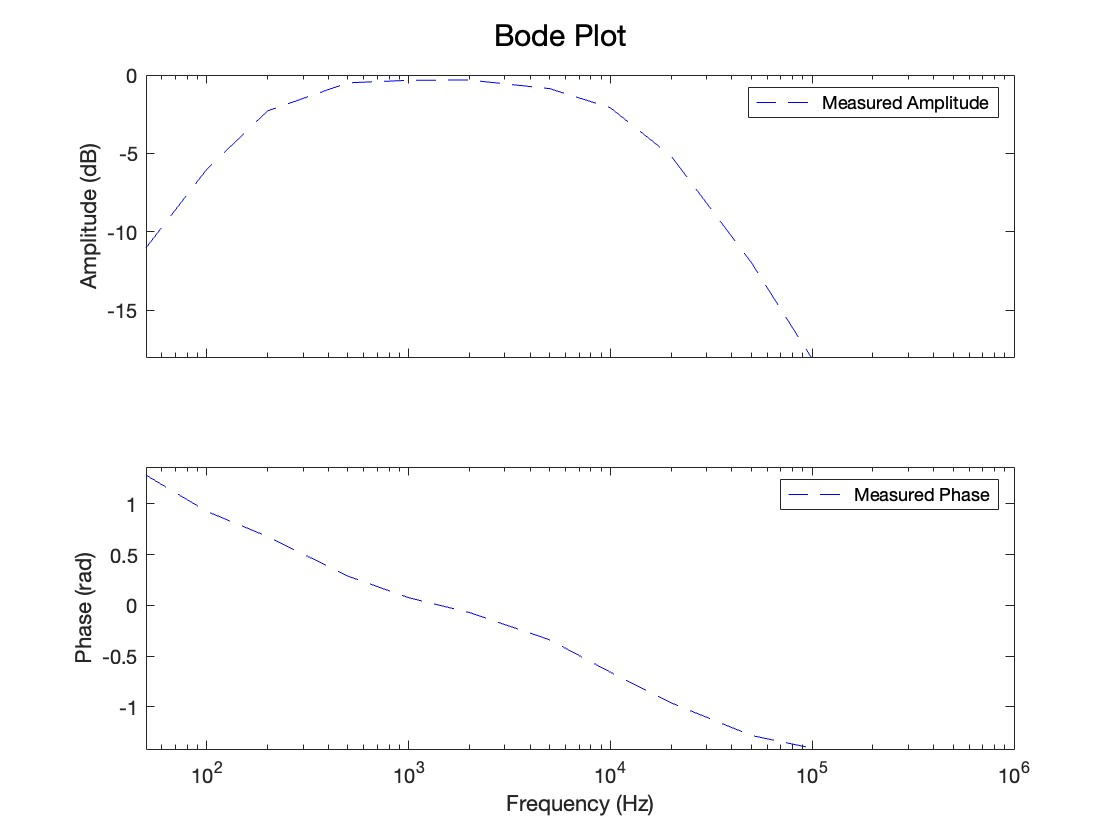
\includegraphics[scale=0.3]{images/bode_plot_bandpass_measured.jpg}
    \caption{Bode plot of measured frequencies, amplitudes and phase shifts of the band pass filter.}
\end{figure}

Furthermore, to obtain the calculated amplitude and phase of the bandpass filter, one must use the appropriate formulas:
\[
    |A_{lo}| = \frac{1}{\sqrt{1+(\omega RC)^2}} \text{ and } \phi_{lo}=-\arctan(\omega RC) \text{ for the low pass filter, and }
\]


\[
    |A_{hi}| = \frac{1}{\sqrt{1+1/(\omega RC)^2}} \text{ and } \phi_{hi}=\arctan\left(\frac{1}{\omega RC}\right) \text{for the high pass filter}
\]


To combine these results, the low and high amplitudes are multiplied, and the phases are added.


\(|A_{total}| = |A_{hi}| * |A_{lo}|\) and \(\phi_{total} = \phi_{hi} + \phi_{lo}\)

Using this methodology, we can compose a graph of calculated amplitude and phase values and compare it to our measured values.

\begin{figure}[H]
    \centering
    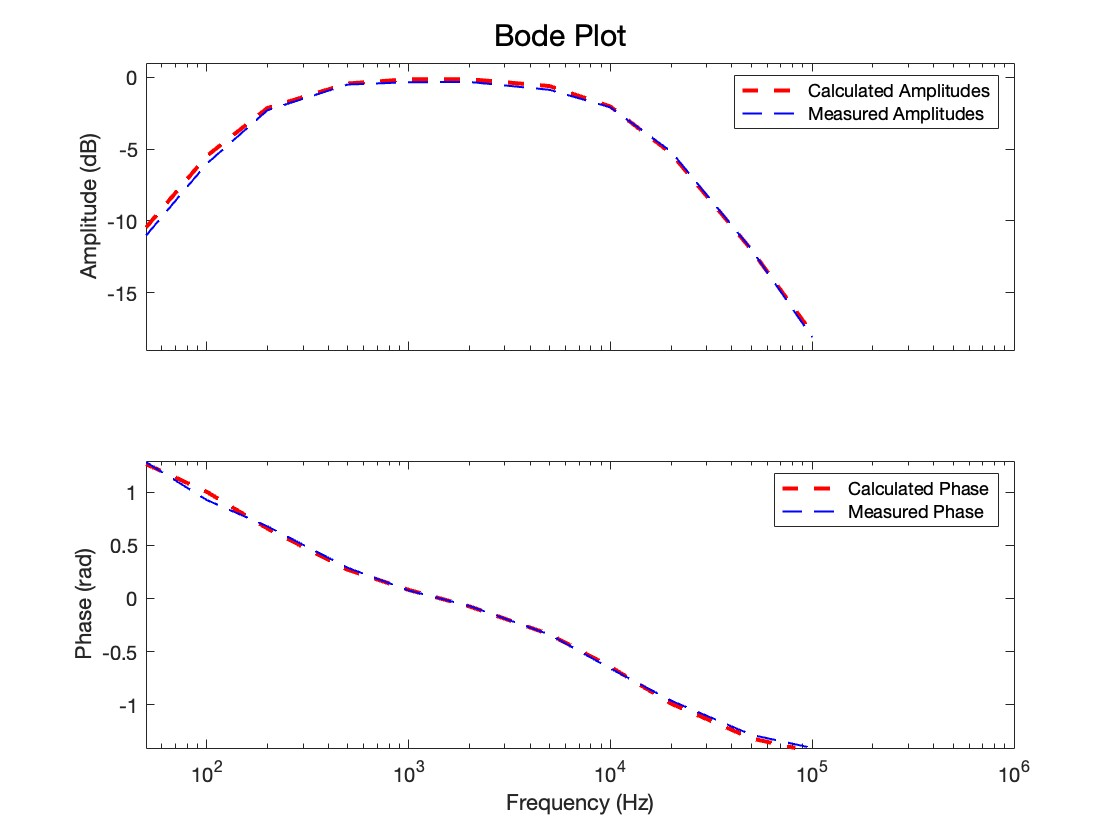
\includegraphics[scale=0.3]{images/bode_plot_bandpass_calculated.jpg}
    \caption{Bode plot of calculated phase and amplitude vs the bode plot of the measured phase and amplitude.}
\end{figure}


We see that the calculated values are very close, almost superimposed. This means that our measured values are as expected, and very close to the nominal amplitude and phase.


To calculate the lower and upper cut-off frequencies, we have to treat each component of the band-pass filter(high and low pass) independently.

We find that for the high-pass component's frequency:
\begin{equation}
    f_{-3dB} = \frac{1}{2\pi \cdot 10^4 \cdot 10^{-7}} = 159.15\text{Hz}
\end{equation}

and for the low-pass component's frequency:

\begin{equation}
    f_{-3dB} = \frac{1}{2\pi \cdot 8200 \cdot 1.5 \cdot 10^{-9}} = 12939\text{Hz}
\end{equation}


The center frequency is then defined as the root of the multiple of both components' frequencies, so:

\begin{equation}
    f_c = \sqrt{f_{c,lo}\cdot f_{c, hi}} = \sqrt{12939 \cdot 159.15} = 1435\text{Hz}
\end{equation}

The bandwidth is simply the difference between the components, so

\begin{equation}
    B = f_{c,lo} - f_{c, hi} = 12939 - 159.15 = 12779.85\text{Hz}
\end{equation}


The phase shift, $\phi$, at the cutoff frequencies is calculated for their respective component:

\begin{equation}
    \phi_{hi}=\arctan\left(\frac{1}{2\pi\cdot12799.85 \cdot 8200 \cdot 1.5 \cdot 10^{-9}}\right) = 45^{\circ}
\end{equation}

And for the low pass component:

\begin{equation}
    \phi_{hi}=-\arctan\left(2\pi \cdot 159.15 \cdot 10^4 \cdot 10^{-7}\right) = -45^{\circ}
\end{equation}

So the total phase shift, by summation:
\begin{equation}
    \phi_{total} = \phi_{hi} + \phi_{lo} = 45^{\circ} - 45^{\circ} = 0^{\circ}
\end{equation}

The results of the measurements are very close to the calculations. The only error that we encounter is from the measurements of the oscilloscope, and due to the passive components used not being completely ideal.


To obtain the Nyquist plot of the band-pass filter, we multiply the transfer functions of the low-pass and high-pass components, and then multiply by the input voltage.

\begin{equation}
    U_R(\omega) = (H_{lo}(j\omega) \cdot H_{hi}(j\omega)) \cdot V_{in}
\end{equation}


The nyquist plot is then drawn using MATLAB.

\begin{figure}[H]
    \centering
    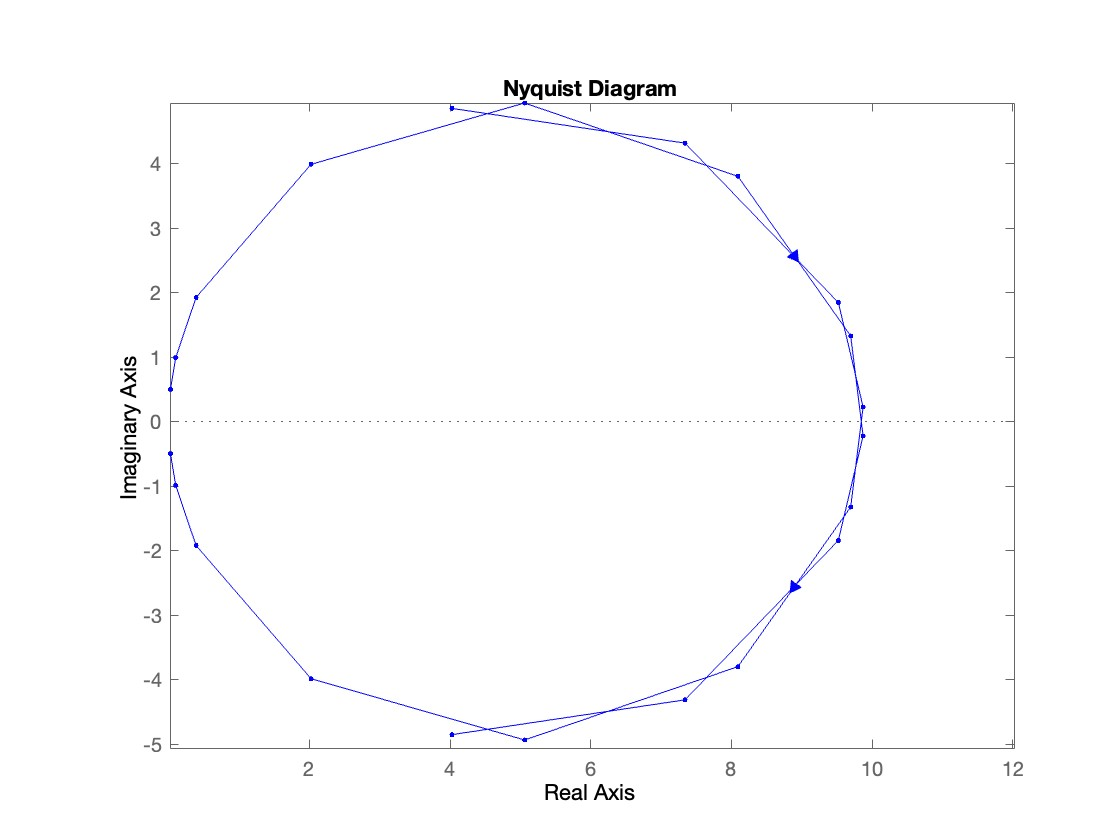
\includegraphics[scale=0.3]{images/nyquist_plot_bandpass.jpg}
    \caption{Nyquist plot of the bandpass filter, composed of the transfer function of the high pass filter and the low pass filter.}
\end{figure}
